\documentclass[t]{beamer}


\usepackage[T1]{fontenc}
\usepackage[utf8]{inputenc}
%\usepackage[ngerman]{babel}
%\usepackage[babel,german=quotes]{csquotes}
\usepackage{graphicx}
\usepackage{color}
\usepackage{import}
% \usepackage{subfig}
%\usepackage[labelformat=empty]{caption}
\newcommand{\themepath}{../latex_templates/theme/}
\subimport{\themepath}{beamerthemefablab-4-3.sty}

\usepackage[font=large,labelfont=bf]{caption}

\begin{document}
% Title page


\date{\today}
\institute{FAU FabLab}
\title[Vorstellung]{Vorstellung des FAU FabLabs}
\author{} % TODO Namen der Vorstellenden eintragen
\frame[plain,c]{\titlepage} % plain-Option deaktiviert Kopf- und Fusszeile


% \captionsetup[subfloat]{labelformat=empty,font=large}

% \frame{\frametitle{Inhalt}\tableofcontents}

\begin{frame}
    \frametitle{Was ist das FabLab?}
    % Was, Wer, Wie, Wo
    \begin{itemize}
        \item Offene Hightech-Werkstatt an der TechFak
        \item Von Studenten für alle
        \item Jeder kann kommen und seine eigenen Ideen umsetzen
        \item Selber machen, lernen wie es geht -- keine Auftragsfertigung\\~
        \item Benutzung zum Selbstkostenpreis: nur Material und Verschleiß\\~
        \item Für dieses Praktikum Abrechnung mit dem Budget möglich,\\
        Ausgaben über Kundenkonto der Gruppe\\~
        \item Sonst: Zahlen und Quittung erhalten
    \end{itemize}

\end{frame}

% \begin{frame}
%     \frametitle{Wo und wie?}
%     \begin{itemize}
%
%
%     \end{itemize}
% \end{frame}
% \section{First Section}
% \subsection{First Subsection}

% \begin{frame}
%     \frametitle{Ausstattung}
%
%     \begin{itemize}
%         \item Lasercutter: schneiden und gravieren
%         \item 3D-Drucker: vom Modell zur Realität
%         \item CNC-Fräse
%         \item CNC-Drehbank
%         \item Platinenherstellung
%         \item Elektrowerkstatt
%         \item Schneideplotter: Folien und Masken schneiden
%     \end{itemize}
%
%     ~\\
%
%%     And some more content
%\end{frame}


\begin{frame}
    \frametitle{Lasercutter: Schneiden und Gravieren}
    \begin{itemize}
        \item Material (vorrätig): Acryl-Kunststoff, Sperrholz, MDF, Pappe
        \item Arbeitsfläche 60$\times$30\,cm, bis ca 10\,mm Dicke, Genauigkeit ungefähr 0,2\,mm
        \item Daten als Vektorzeichnung (Inkscape, Corel Draw, CAD (.DXF), ...)
    \end{itemize}

    \bigskip

    \bigskip
    \begin{center}
        
\includegraphics[height=6cm]{../img/SquareGears.pdf}
        
\includegraphics[height=6cm]{../img/pfeil.pdf}
        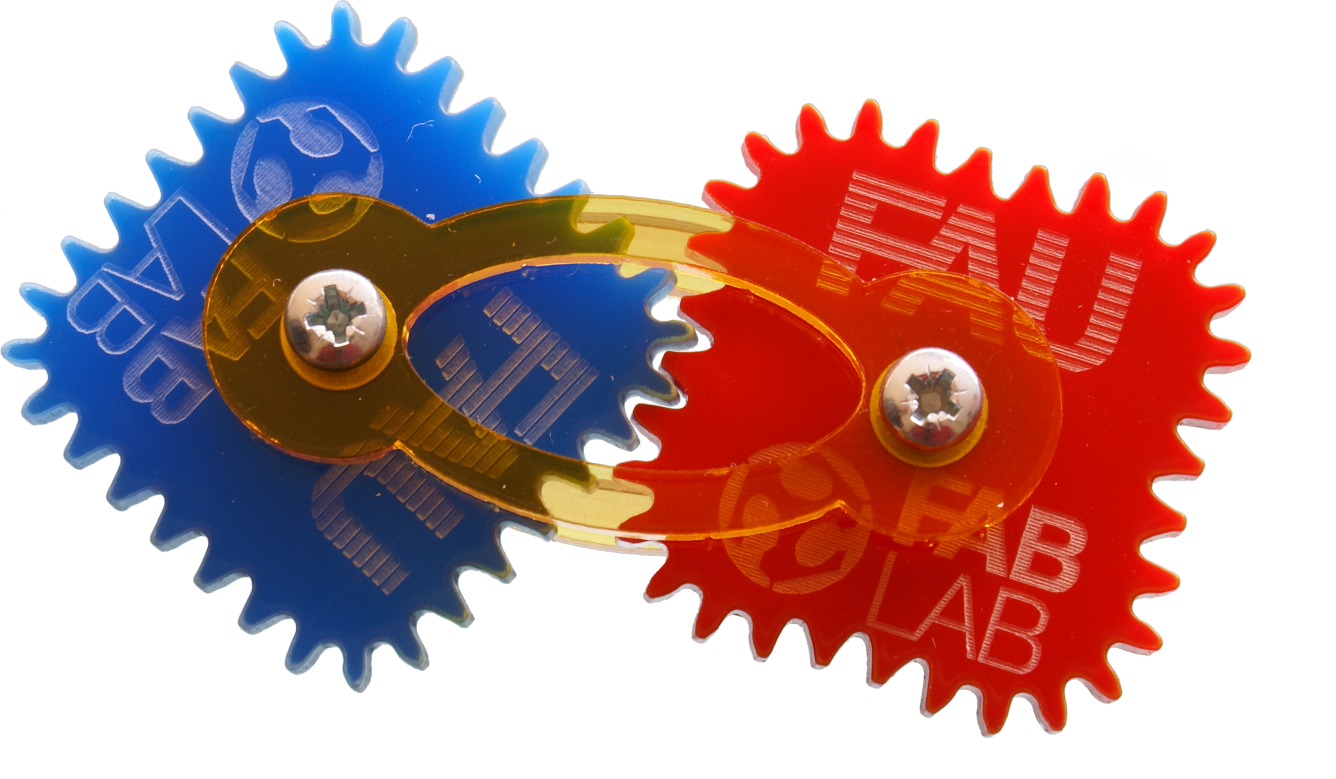
\includegraphics[height=6cm]{../img/zahnraeder2b-skaliert.png}
    \end{center}

\end{frame}


\begin{frame}{Lasercutter: Beispiel Holz}
    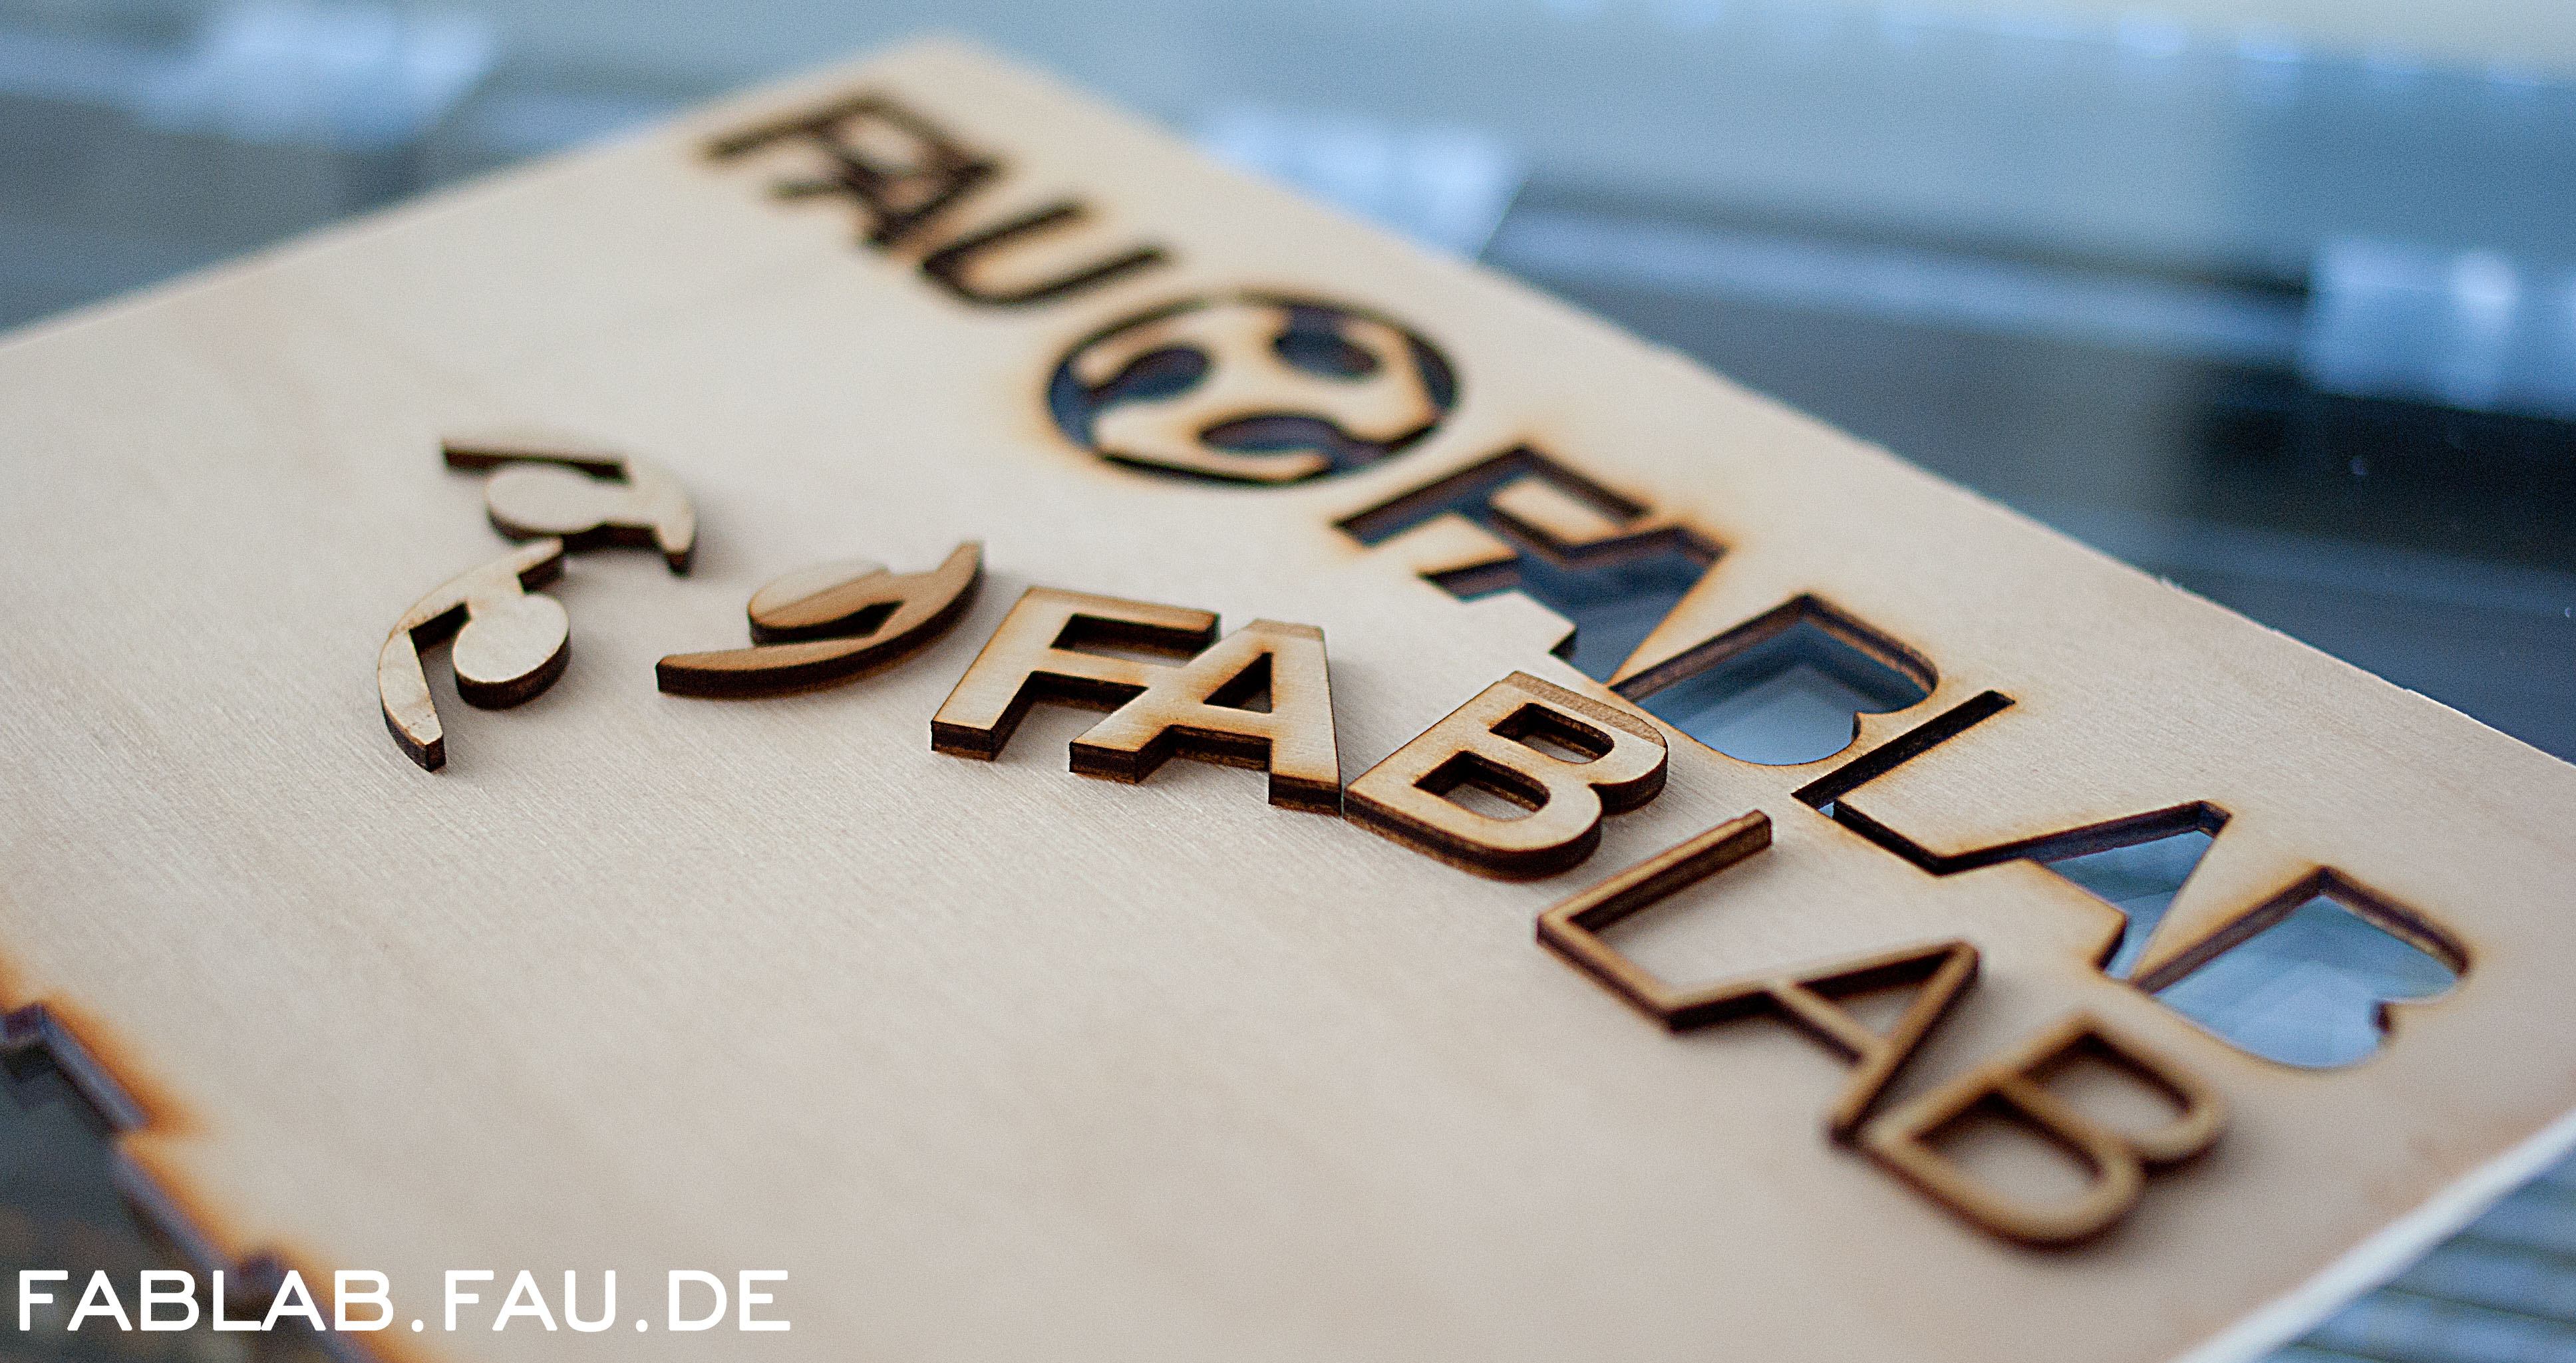
\includegraphics[width=\textwidth]{../img/lasercut-holz.jpg}
\end{frame}
\begin{frame}{Lasercutter: Beispiel Kunststoff}
    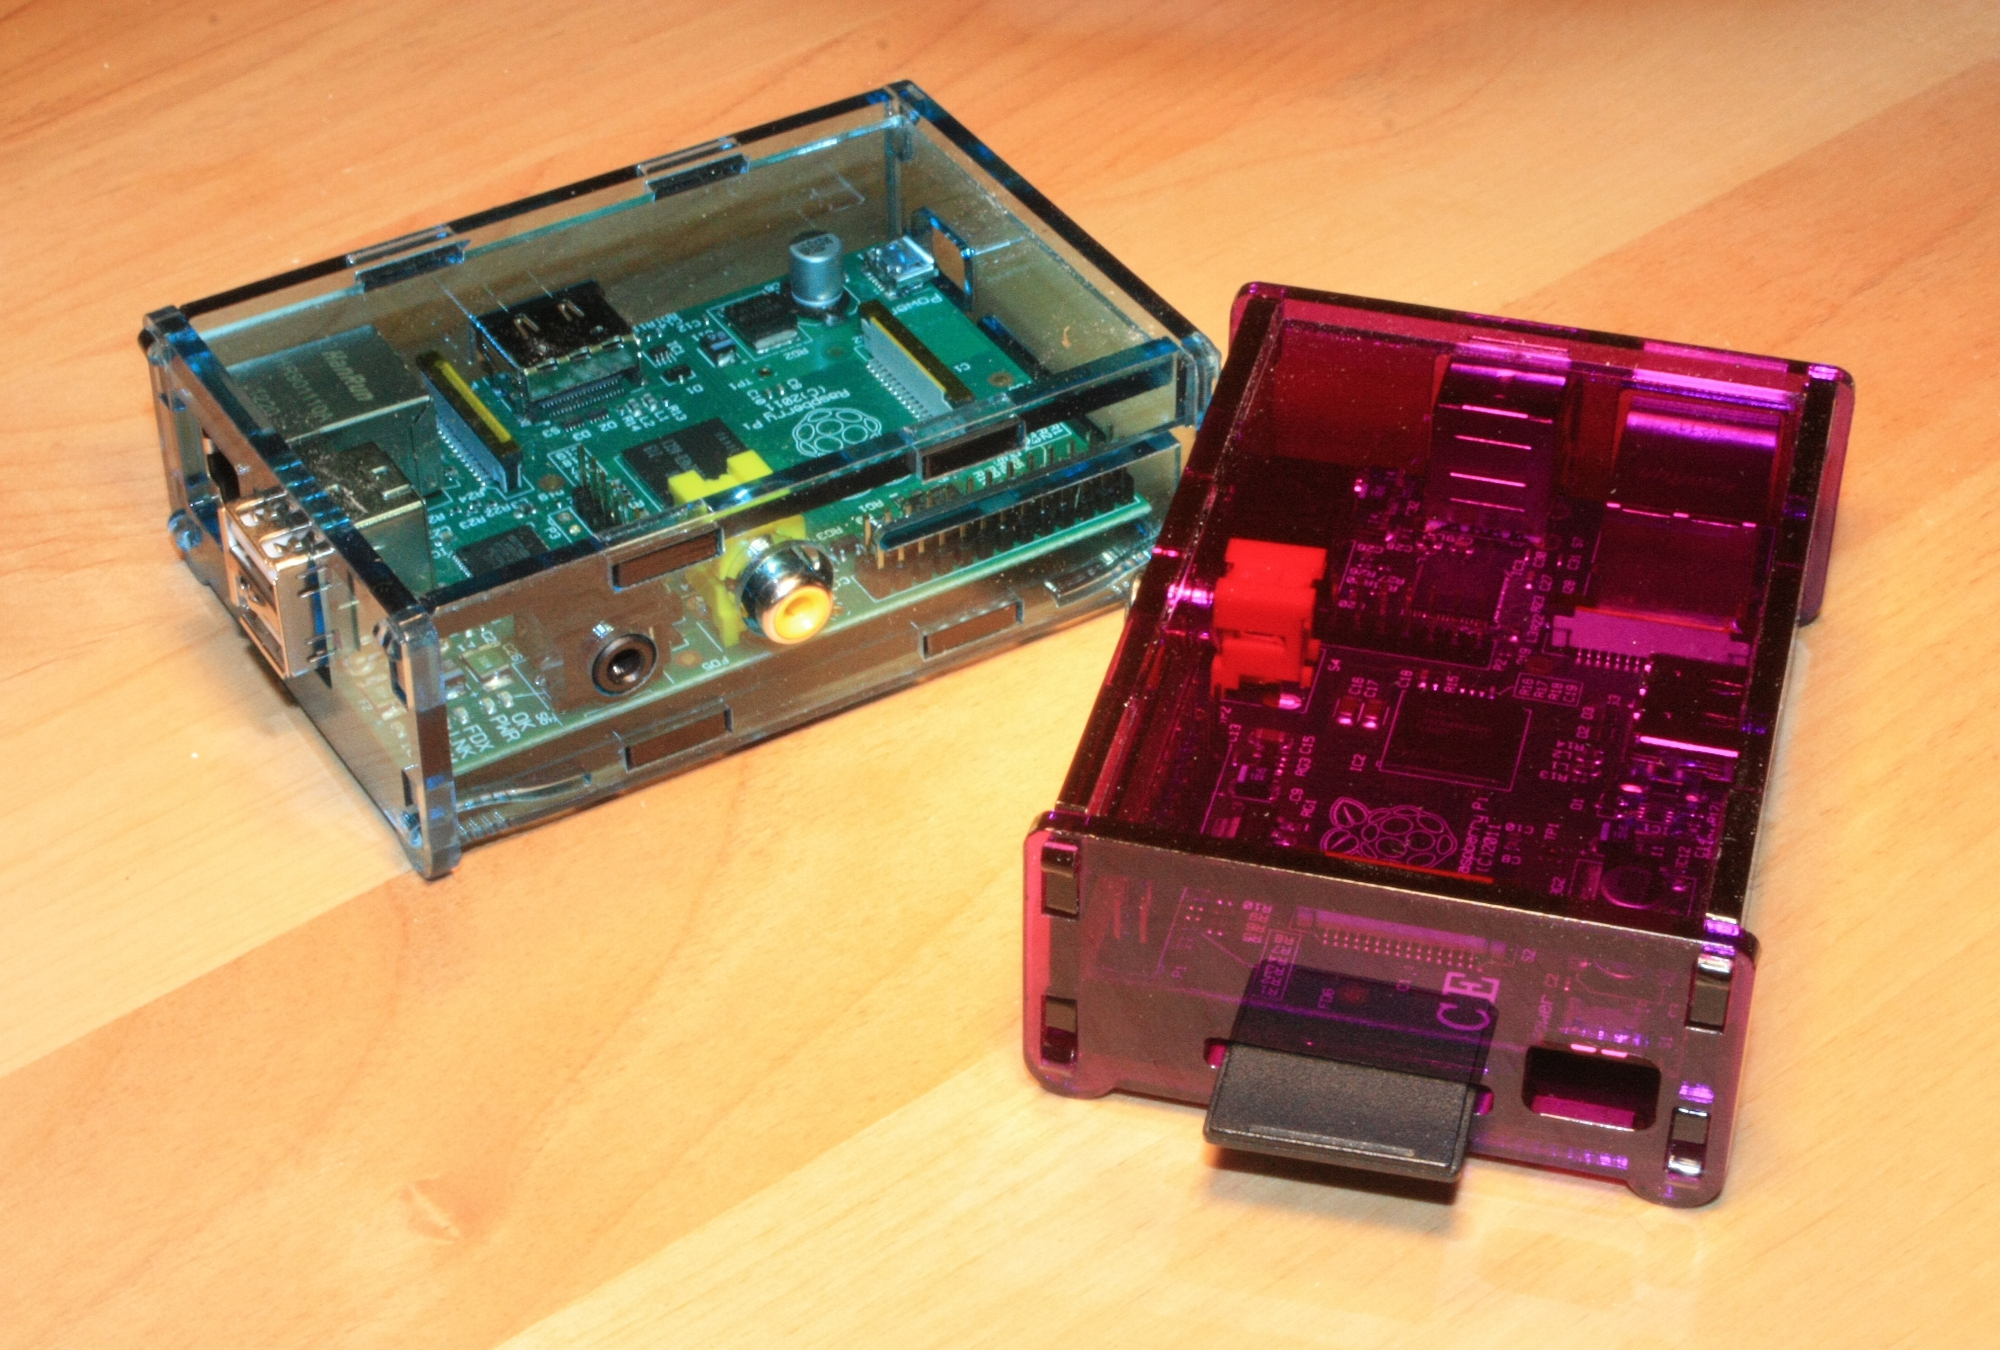
\includegraphics[width=\textwidth,clip,trim=0 5cm 0 2cm]{../img/lasercut-kunststoff.jpg}
\end{frame}

\begin{frame}
    \frametitle{3D-Drucker: vom CAD-Modell zur Realität}
    \begin{itemize}
        \item Kunststoff: PLA oder ABS
        \item Maximale Baugröße 13$\times$19$\times$8\,cm
        \item Nicht alles ist sinnvoll druckbar - vorher nachfragen!
        \item Daten als 3D-Modell (.STL)
    \end{itemize}
    \bigskip
    \begin{tabular}{lll}
        {\color{faublue} Name} & {\color{faublue} Baugröße} & {\color{faublue} Min. Schichthöhe}\\
        %RepRap & 13x19x8\,cm & 0.5\,mm & 2\,mm \\
        Ultimaker 2 & 23x22x20\,cm & \textasciitilde0.02\,mm \\
        Ultimaker & 21x21x20\,cm & \textasciitilde0.1\,mm \\
        MakerBot Replicator 2X & 25x16x15\,cm & 0.1\,mm \\
    \end{tabular}
    \bigskip
    \begin{center}
    ~\\
        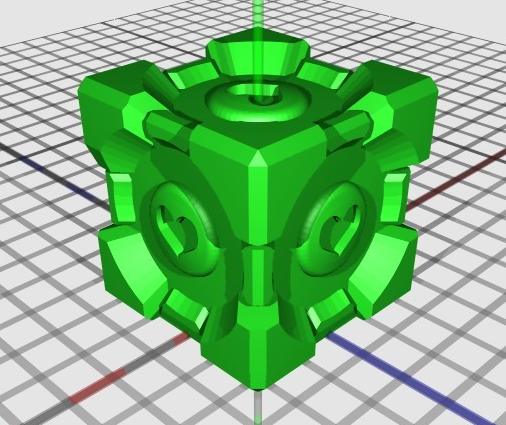
\includegraphics[height=6cm]{../img/companioncube_render.png}
        
\includegraphics[height=6cm]{../img/pfeil.pdf}
        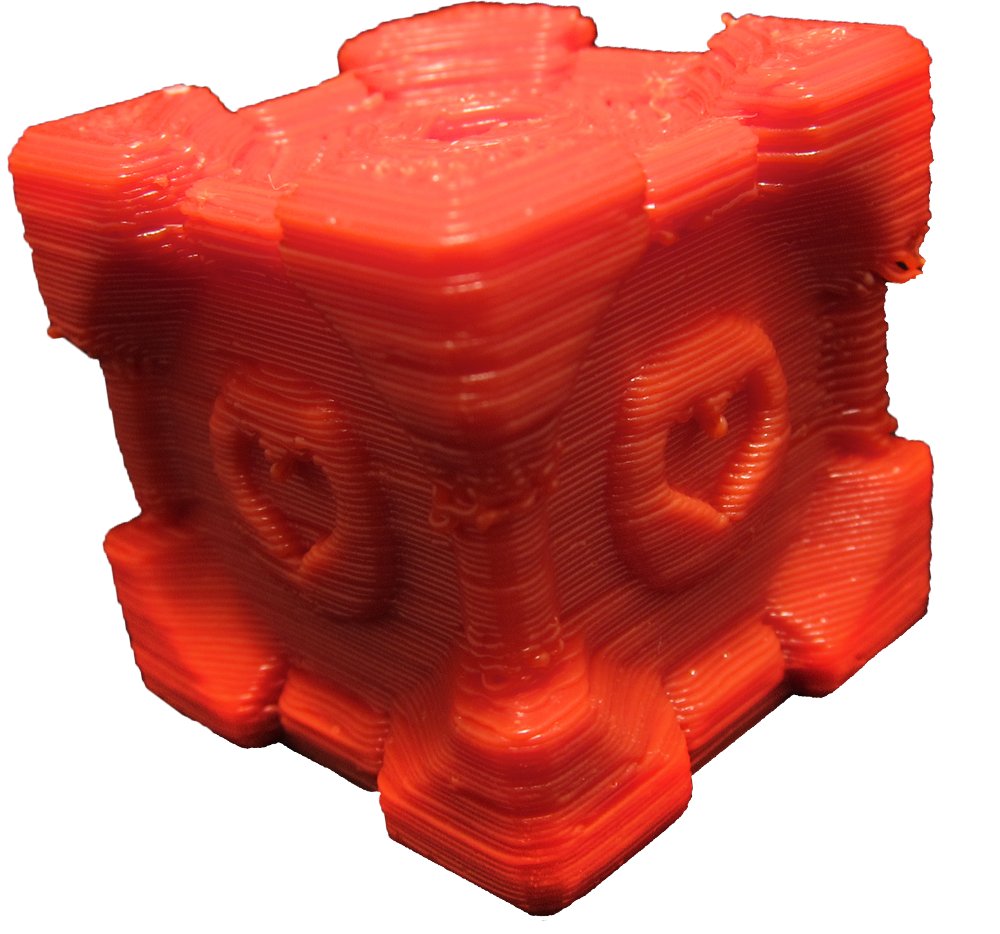
\includegraphics[height=6cm]{../img/companioncube.png}
    \end{center}
\end{frame}

\begin{frame}
    \frametitle{CNC-Fräse}
    \begin{itemize}
        \item Material: Aluminium, Stahl, Holz, Kunststoff
        \item Werkstücke bis etwa 50$\times$30$\times$10\,cm
        \item Genauigkeit besser als 0.1\,mm
        \item Daten als 2D-Zeichnung oder 3D-CAD-Modell (DXF, STL, STEP, IGES, ...)
        \item Aktuell im Umbau.
    \end{itemize}
    \begin{center}
    ~\\
    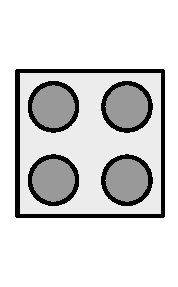
\includegraphics[height=6cm]{../img/legozeichnung.pdf}
    
\includegraphics[height=6cm]{../img/pfeil.pdf}
    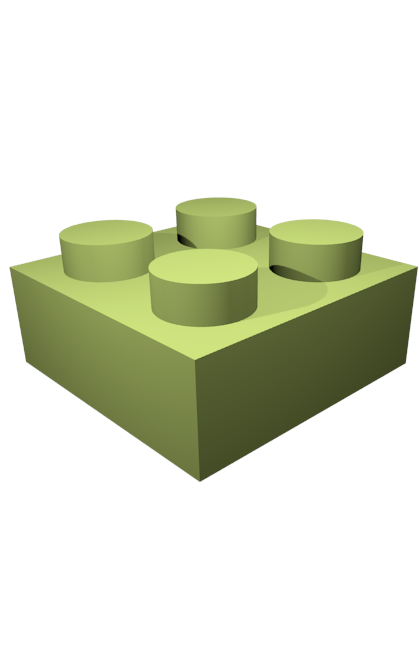
\includegraphics[height=6cm]{../img/fraese-lego-3d.png}
    
\includegraphics[height=6cm]{../img/pfeil.pdf}
    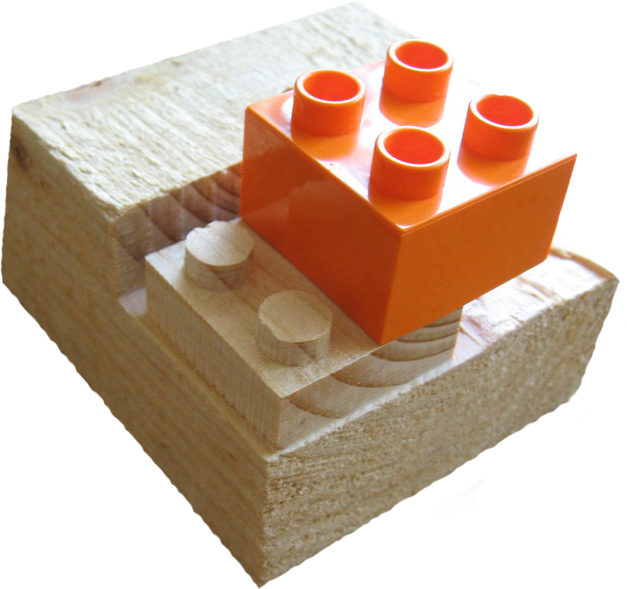
\includegraphics[height=6cm]{../img/fraese-lego.png}

    \end{center}
\end{frame}

\begin{frame}
    \frametitle{CNC-Drehbank}
    \begin{itemize}
        \item Material: z.B. Aluminium, POM
        \item Noch im Testbetrieb
    \end{itemize}
        \begin{center}
    ~\\
        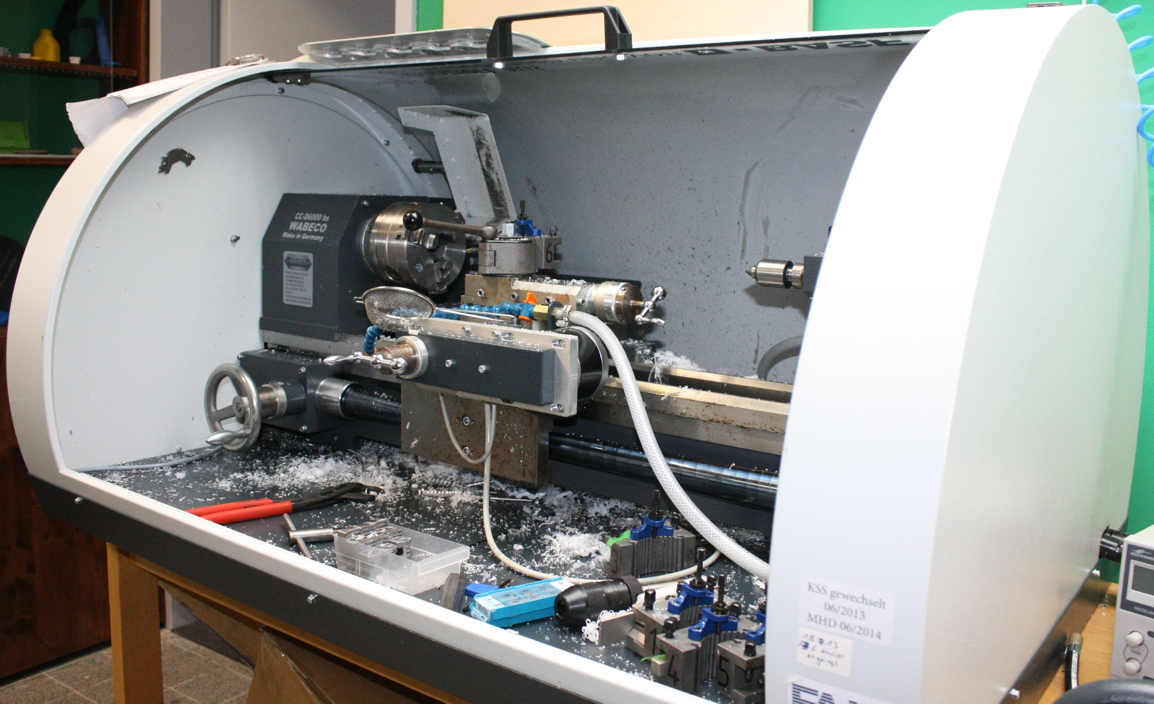
\includegraphics[height=8cm]{../img/drehbank.png}
        ~~~
        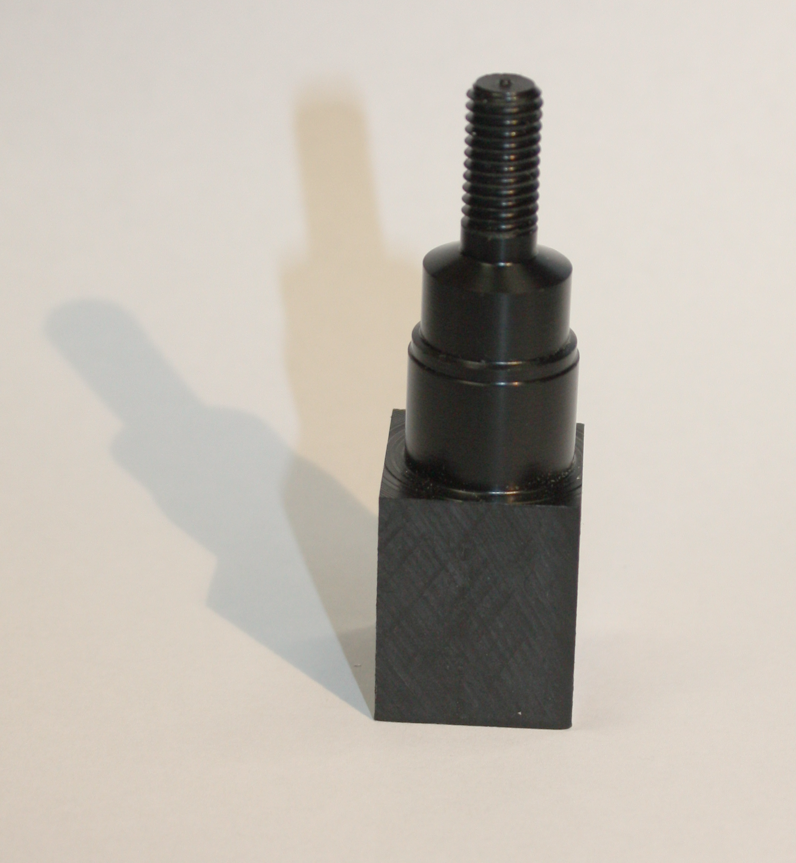
\includegraphics[height=8cm]{../img/drehstueck.png}
    \end{center}
\end{frame}

\begin{frame}
    \frametitle{Elektrowerkstatt}
    \begin{itemize}
        \item Lötkolben, Oszi usw.
        \item Platinen selber fertigen:\\
            16$\times$10\,cm, ein- oder doppelseitig -- technische Vorgaben beachten
        \item Bauteileverkauf (ca. 350 gängige Typen)
    \end{itemize}
        \begin{center}
    ~\\
        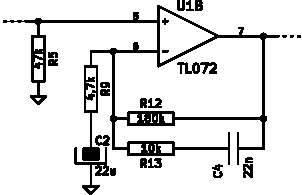
\includegraphics[height=6cm]{../img/schaltplan.pdf}
        
\includegraphics[height=6cm]{../img/pfeil.pdf}
        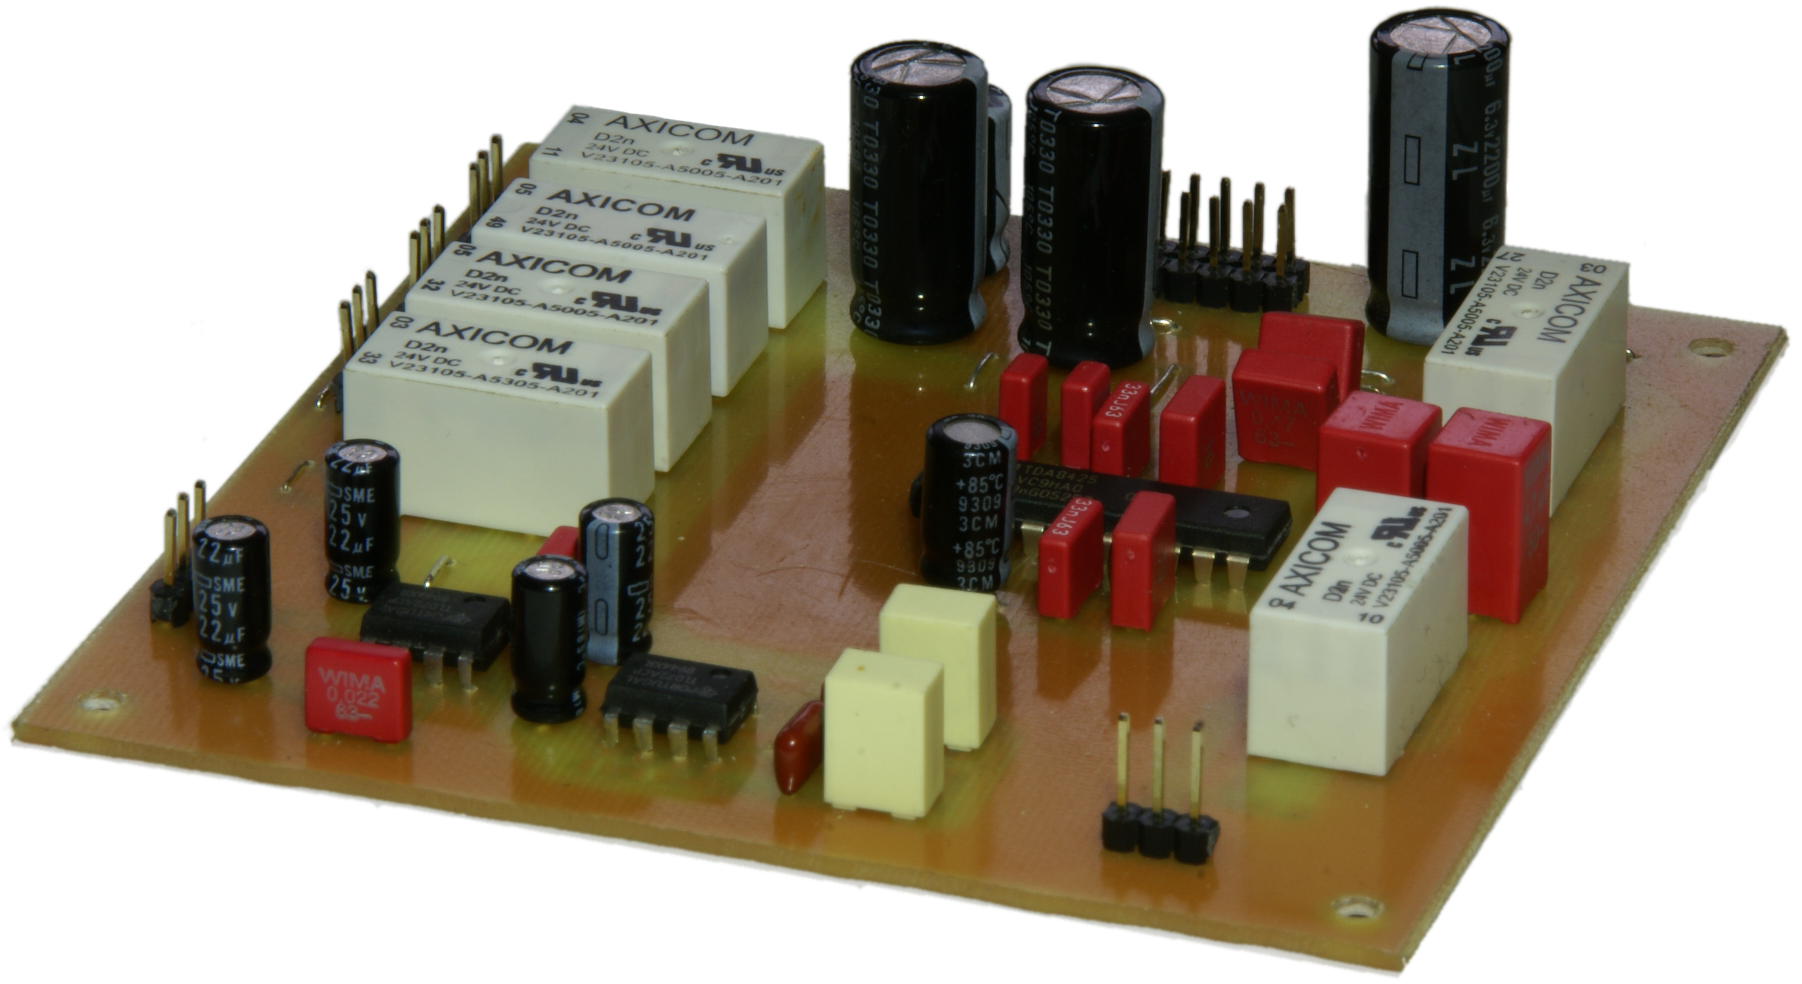
\includegraphics[height=6cm]{../img/platine_perspektivisch.png}
    \end{center}
\end{frame}

\begin{frame}
    \frametitle{weitere Ausstattung}
    \begin{itemize}
        \item Werkzeug wie Schraubendreher, Feilen, Stichsäge etc.
        \item Folienschneider
        \item Standbohrmaschine
        \item Nähmaschine
        \item Grundausstattung an CAD-Software
        \item Grundstock an Material für alle Geräte
    \end{itemize}
    \begin{center}
        ~\\

        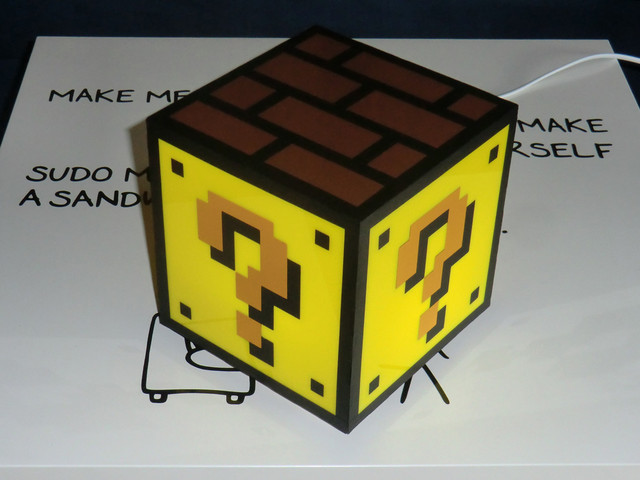
\includegraphics[height=7cm]{../img/mariolampe.jpg}
        \hspace{1em}
        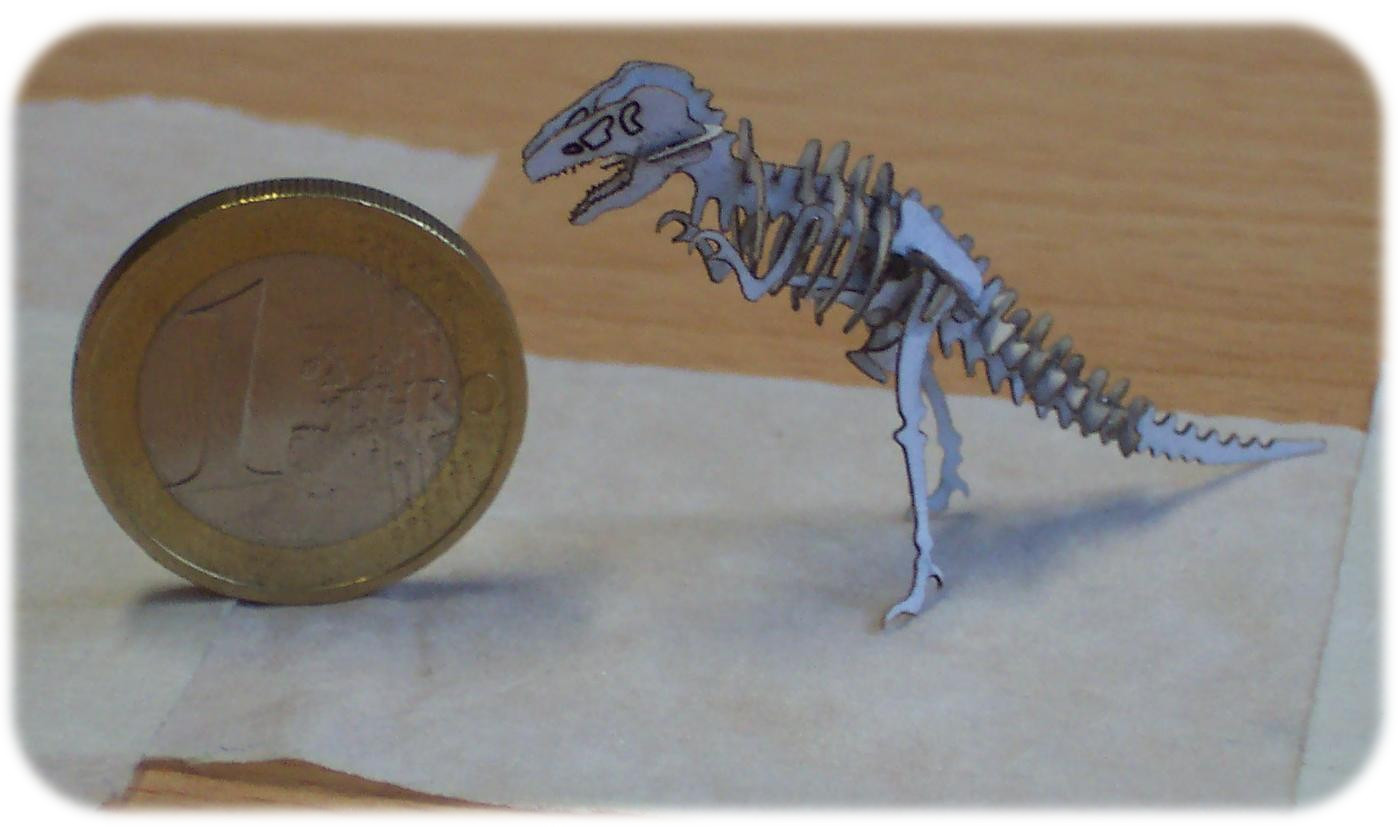
\includegraphics[height=7cm]{../img/tinysaur.jpg}
    \end{center}
\end{frame}

\begin{frame}
    \frametitle{Interesse?}

    \begin{itemize}
        \item Ort: Hörsaalgebäude, beim unteren Ausgang H8/H9 (Erwin-Rommel-Straße 60, Raum U1.239)
        \item Öffnungszeiten: \\Ab zweiter Semesterwoche regelmäßig OpenLab/SelfLab
        % \item Workshops: Löten (Anfänger/Fortgeschrittene), 3D-Modellierung, usw.
        \item Weitere Termine auf {\color{blue} https://fablab.fau.de/termine}
    \end{itemize}
    ~\\
    Merchandising
    \begin{itemize}
        \item Mitgebrachte Werkstücke ansehen
        \item Flyer mitnehmen
    \end{itemize}
    ~\\
    Fragen?
    \begin{itemize}
        \item Website {\color{blue} https://fablab.fau.de}
        \item E-Mail {\color{blue} kontakt@fablab.fau.de}
        \item Einfach vorbeikommen oder jetzt nachfragen
    \end{itemize}
\end{frame}

%
% \subsection{Second Subsection}

% \begin{frame}[plain]
%     \begin{center}
%         %\color{white}
%         %\footnotesize
%         ~\\~\\~\\~\\~\\~\\~\\~\\~\\
%         END
%     \end{center}
% \end{frame}

\end{document}
